\documentclass{article}

\usepackage[utf8]{inputenc}
\usepackage{amssymb}
\usepackage{amsmath}
\usepackage{mathabx}
\usepackage{dcolumn}
\usepackage{geometry}
\usepackage{breqn}
\usepackage{graphicx}
\usepackage{float}
\usepackage{mathrsfs}
\usepackage{array}
\usepackage{caption}
\usepackage{subcaption}
\usepackage[spanish,es-lcroman]{babel}
\decimalpoint
\usepackage{enumerate}
\usepackage{nicefrac} 
\usepackage[most]{tcolorbox}
\usepackage{tcolorbox} % For solution boxes
%\decimalpoint
\setlength\parindent{0pt}
\usepackage{enumitem}
\newcommand*{\QED}{\hfill\ensuremath{\blacksquare}}
%\usepackage{authblk}
\selectlanguage{spanish}
\geometry{letterpaper, margin=1in}
\pagestyle{headings}
\usepackage{amsthm} 
\newtheorem{theorem}{Teorema}[section]
\newtheorem{corollary}{Corolario}[theorem]
\newtheorem{lemma}[theorem]{Lema}
\theoremstyle{remark}
\newtheorem*{remark}{Considere}
\DeclareUnicodeCharacter{2212}{-}
\usepackage{epigraph}
\usepackage{xcolor}

\renewcommand{\thesubsection}{\arabic{subsection}}

\usepackage[backend=biber, style=apa]{biblatex}
\addbibresource{bib/ref_entrega1.bib}
\usepackage{tikz}
\usepackage{hyperref}

\tcbset{colback=blue!10, 
    %colframe=green!45!black!20, 
    colframe=blue!70!black!70, 
    title=Soluci\'on,
    fonttitle=\bfseries,  
    coltitle=white,
    standard jigsaw, opacityback=50, arc=0mm, breakable} 

\newcommand{\ubar}[1]{\text{\b{$#1$}}}
 
\theoremstyle{definition}
\newtheorem{definition}{Definici\'on}[section]

\title{\textbf{Macroeconom\'ia Avanzada de Largo Plazo} \\ \textbf{Taller 1 - Parte Grupal}}

\author{Jhoan Sebasti\'an Fuentes Hern\'andez \and Nicolas Lozano Huertas}
\date{2025-10}

\begin{document}
\maketitle
\vspace{-1 cm}

\section*{[100 puntos] Parte 2: Trabajo de Investigaci\'on}

\subsection{[30 puntos] Un ejemplo de teor\'ia aplicada}

Lea el art\'iculo ``Achieving Scale Collectively'' por Bassi et al.\ (2022). Responda los siguientes puntos:

\begin{enumerate}[label= (\roman*)]
\item Resuma en sus palabras el art\'iculo $(<200\text{ palabras})$. Es decir, resuma qu\'e cree usted que el art\'iculo dice. Note que los modelos de lenguaje pueden solamente resumir lo que el art\'iculo dice.

    \begin{tcolorbox}

    El artículo “Achieving Scale Collectively” (Bassi et al., 2022) analiza cómo, en países en desarrollo, las microempresas —empresas con poca capacidad para comprar tecnología moderna costosa e indivisible— pueden acceder a maquinaria avanzada mediante mercados informales de alquiler. Basado en encuestas en Uganda , se observa que, aunque pocas firmas adquieren equipos costosos, la mayoría utiliza el arriendo, compartiendo la capacidad excedente en clústeres geográficos. Los autores desarrollan y calibran un modelo de equilibrio que incorpora fricciones en el mercado de alquiler (medidas por un costo transaccional, $\tau$) y en el mercado laboral, demostrando que la reducción de $\tau$ mejora la asignación de capital, incrementa la mecanización y eleva la productividad. Así, ``alcanzar escala colectivamente'' surge como un mecanismo esencial para superar la indivisibilidad del capital en microempresas.
        
    \end{tcolorbox}


\item Describa en sus palabras los resultados emp\'iricos que motivan las elecciones del modelo te\'orico.

     \begin{tcolorbox}

     Los datos revelan:
    \begin{enumerate}
        \item Existencia de talleres extremadamente pequeños (pocas decenas de trabajadores) concentrados en clústeres informales.
        \item Máquinas eléctricas costosas e indivisibles, con capacidad superior a las necesidades de una sola firma.
        \item Un marcado mercado de arriendo intraclúster, donde pocas empresas propietarias rentan sus equipos a otras.
        \item Presencia de costos de transacción (tiempo de viaje, congestión, etc.) que, pese a ello, no impiden que el arriendo impulse la mecanización, productividad y calidad.
    \end{enumerate}
        
    \end{tcolorbox}

\item Para cada uno de esos resultados, describa c\'omo se conecta con la teor\'ia. En particular, describa qu\'e tipo de supuestos de comportamiento y supuestos de equilibrio surgen a partir de los hechos estilizados.

     \begin{tcolorbox}

     A partir de los hechos empíricos se derivan los siguientes supuestos teóricos:
    \begin{itemize}
        \item \textbf{Indivisibilidad del capital:} La necesidad de máquinas de gran capacidad justifica que pequeñas firmas dependan de mecanismos colectivos al no tener la capacidad de comprar tecnolog\'ia propia.
        \item \textbf{Mercado de alquiler con fricciones:} Se incorporan costos de transacción (transporte, espera) acordes con lo observado.
        \item \textbf{Rendimientos crecientes a escala limitados por fricciones:} Compartir maquinaria aumenta la productividad, determinándose en equilibrio precios de arriendo y asignación de uso.
        \item \textbf{Heterogeneidad en capacidades y financiamiento:} Variaciones en gestión y costos explican la disparidad empírica en tamaño y habilidad.
    \end{itemize}
        
    \end{tcolorbox}

\item En qu\'e se aleja este modelo del modelo neocl\'asico de crecimiento? La pregunta es por las diferencias en t\'erminos conceptuales, pero haga referencia a los objetos te\'oricos para responder a esta pregunta.

     \begin{tcolorbox}

     El modelo se diferencia del neoclásico al:
    \begin{enumerate}
        \item Incorporar capital indivisible y capacidad ociosa significativa.
        \item Reconocer fricciones en mercados laborales, financieros y de demanda.
        \item Destacar el rol del arriendo intraclúster como mecanismo informal de cooperación.
        \item Considerar una distribución de tamaños dominada por pequeñas firmas, en contraposición al modelo de “firma representativa.”
    \end{enumerate}
        
        
    \end{tcolorbox}

\item Describa intuitivamente los resultados te\'oricos del modelo. C\'omo se conectan estos con la evidencia emp\'irica? Qu\'e tipo de conclusiones se pueden obtener de estos resultados?

     \begin{tcolorbox}
        El modelo deriva funciones umbral, $\hat{x}(z)$ y $\hat{z}(x)$, que determinan qué gestores compran máquinas y cuáles optan por el arriendo. La introducción de $\tau$ eleva el costo marginal para arrendatarios, reduciendo la proporción capital-trabajo ($K/L$) respecto a los propietarios. Se predice que una reducción en $\tau$ incrementa la mecanización, productividad y producción total. Los mecanismos clave son:
        \begin{itemize}
            \item \textbf{Escala efectiva:} Compartir maquinaria disminuye los costos fijos de equipos de gran envergadura.
            \item \textbf{Reasignación de capital:} Diferencias en financiamiento permiten que unos adquieran equipos y otros los utilicen, optimizando el uso de recursos.
        \end{itemize}
        Encuestas en Uganda confirman que, pese a costos de transacción (con $\tau \approx 0.43$), el mercado de arriendo impulsa la mecanización y mejora la productividad, validando que “alcanzar escala colectivamente” es clave para superar la indivisibilidad del capital en microempresas.

    \end{tcolorbox}

\end{enumerate}

\subsection{[70 puntos] Trabajo de investigaci\'on}

El propósito de este problema es identificar una dimensión específica del proceso de crecimiento económico, explorar su relevancia empírica y comenzar a desarrollar un marco teórico para analizarla que extienda los modelos teóricos simples que estaremos cubriendo durante el curso. Este ejercicio está diseñado como un primer paso hacia el proyecto final del curso.

\subsubsection{[10 puntos] Elección de tema y justificación}

Identifique un tema relacionado con el crecimiento económico. Trate de ser lo más preciso posible, temas generales (e.g. el capital humano) le harán muy difícil aterrizar sus ideas. Escriba un párrafo explicando por qué este tema es importante para entender el crecimiento económico. Incluya al menos una referencia a un artículo, un hecho estilizado o una tendencia histórica que respalde su elección.



\begin{tcolorbox}
    
\textbf{El auge del sector servicios: oportunidad para el cambio técnico complementario}


El tema que proponemos investigar es cómo la menor susceptibilidad a la automatización en labores cognitivas y sociales (con "rostro humano") puede volverse un mecanismo generador de crecimiento inclusivo. Entendido este como el crecimiento que emplea una tecnología en la que el capital no elimina por completo el trabajo, sino que se complementan. 
Encontramos una primera evidencia sugestiva de que la hipótesis puede cumplirse.
A partir de las bases de datos (O*NET y las encuestas Occupational Employment and Wage Statistics (OEWS) Survey de Estados Unidos) encontramos correlaciones positivas entre la intensidad de actividades cognitivas ($r=0.56$) y las sociales ($r=0.31$) con unos valores salariales más altos. En contraste, las actividades técnicas (uso de maquinarias, trabajos manuales,...) fácilmente automatizables tienen correlaciones negativas relevantes ($r=-0.25$). El patrón empírico podría sugerir que el progreso tecnológico reciente, podría/pudo estar produciendo complementariedades específicas en el sector servicios de la economía con trabajo humano intensivo en conocimiento y habilidades sociales.


Esta dimensión resulta clave para entender las dinámicas del crecimiento económico actual, ya que plantea una ruta de desarrollo alternativa en un escenario donde la manufactura —tradicionalmente considerada el ``escalador automático'' hacia mayores niveles de ingreso— está viendo reducida su capacidad de generar empleos de calidad debido a la automatización. Es lo que Rodrik bautizó como ``Desindustrialización Prematura''. Según Restrepo (2024), la incorporación de robots industriales ha disminuido notablemente la participación laboral en el sector manufacturero, sobre todo entre trabajadores menos calificados, con una caída de alrededor del 20\% en el empleo de producción. 



Este aspecto adquiere especial relevancia a la luz del hallazgo de Fujiwara y Matsuyama (2024), quienes señalan que la desindustrialización prematura —fenómeno en el que países en desarrollo alcanzan su pico manufacturero con niveles de ingreso significativamente más bajos que los observados históricamente en economías avanzadas— no se debe principalmente a la hiperglobalización, como proponía Rodrik (2016), sino a brechas tecnológicas sectoriales que hacen inevitable una transición más temprana hacia los servicios. En este marco estructural, la menor susceptibilidad a la automatización y la mayor complementariedad tecnológica de las actividades cognitivas y sociales podrían facilitar un tipo de crecimiento económico que combine dinamismo productivo con mejor distribución del ingreso. Este proceso operaría a través de un mecanismo de causación circular acumulativa, en el que interactúan el capital humano específico, la adopción de tecnologías complementarias y aumentos salariales sostenidos.
\end{tcolorbox}

\subsubsection{[10 puntos] Medición y Exploración de Datos}

Identifique una base de datos o una variable proxy que permita medir la dimensión elegida. Describa la fuente de datos, las variables principales y cualquier limitación de la información. Tenga en cuenta que la mayoría de artículos empíricos publicados después de 2010 proveen paquetes de replicación que pueden ser buena fuente de información. Calcule estadísticas descriptivas básicas (por ejemplo, media, varianza) para las variables clave y preséntelas en una tabla. Genere al menos una visualización (por ejemplo, un gráfico de dispersión, un histograma, unas series de tiempo) que muestre la relación entre su dimensión y otros indicadores clave de crecimiento (por ejemplo, crecimiento del PIB, TFP o tasas de inversión).


\begin{tcolorbox}
    
\textbf{Fuentes de Datos y Variables Proxy}

Para medir empíricamente la complementariedad trabajo-capital en servicios intensivos en habilidades cognitivas y sociales, utilizamos un enfoque de microdatos ocupacionales. Las principales fuentes de datos son:

\paragraph{1. Base de Datos Ocupacional O*NET (Occupational Information Network)}
\begin{itemize}
\item \textbf{Fuente}: Departamento de Trabajo de EE.UU.
\item \textbf{Cobertura}: Más de 800 ocupaciones detalladas representativas de toda la economía estadounidense
\item \textbf{Variables clave}:
  \begin{itemize}
  \item \texttt{Element Name}: Tipo específico de actividad laboral (e.g., ``Analyzing Data or Information'')
  \item \texttt{Scale Name}: Dimensión evaluada (``Importance'' o ``Level'')
  \item \texttt{Data Value}: Valoración cuantitativa en escala 1-5 de cada actividad
  \item \texttt{N}: Número de evaluadores por ocupación y actividad
  \end{itemize}
\item \textbf{Método de recolección}: Encuestas a incumbentes y expertos ocupacionales
\end{itemize}

\paragraph{2. Occupational Employment and Wage Statistics (OEWS)}
\begin{itemize}
\item \textbf{Fuente}: Bureau of Labor Statistics (BLS), panel 2021-2023
\item \textbf{Cobertura}: 178,358 observaciones, 831 ocupaciones detalladas
\item \textbf{Variables clave}:
  \begin{itemize}
  \item \texttt{a\_mean}: Salario medio anual por ocupación
  \item \texttt{a\_median}: Salario mediano anual por ocupación
  \item \texttt{tot\_emp}: Empleo total por ocupación
  \end{itemize}
\item \textbf{Método de recolección}: Encuesta semestral a establecimientos
\end{itemize}

\textbf{Operacionalización de Variables y Construcción de Índices}

\paragraph{1. Categorización de Actividades Laborales}
Para operacionalizar el concepto de ``susceptibilidad a la automatización'', clasifico las actividades laborales en cuatro categorías según su naturaleza:

\begin{verbatim}
categorias_actividades = {
    `Cognitivas': [
        `Thinking Creatively', 'Making Decisions and Solving Problems',
        `Analyzing Data or Information', 'Developing Objectives and Strategies',
        `Interpreting the Meaning of Information for Others',
        `Updating and Using Relevant Knowledge'
    ],
    `Sociales': [
        `Establishing and Maintaining Interpersonal Relationships',
        `Resolving Conflicts and Negotiating with Others',
        `Assisting and Caring for Others',
        `Coaching and Developing Others',
        `Communicating with Persons Outside Organization',
        `Communicating with Supervisors, Peers, or Subordinates'
    ],
    `Técnicas': [
        `Operating Vehicles, Mechanized Devices, or Equipment',
        `Drafting, Laying Out, and Specifying Technical Devices',
        `Repairing and Maintaining Electronic Equipment',
        `Repairing and Maintaining Mechanical Equipment',
        `Controlling Machines and Processes'
    ],
    `Rutinarias': [
        `Performing Administrative Activities',
        `Documenting/Recording Information',
        `Processing Information',
        `Performing General Physical Activities',
        `Handling and Moving Objects'
    ]
}
\end{verbatim}

\paragraph{2. Intensidad Categórica por Ocupación}
Para cada ocupación $j$, calculo la intensidad media de cada categoría $c$:

\begin{align}
I_{j,c} = \frac{1}{n_c} \sum_{i \in c} v_{i,j}
\end{align}

Donde:
\begin{itemize}
\item $I_{j,c}$ es la intensidad de la categoría $c$ en la ocupación $j$
\item $n_c$ es el número de actividades en la categoría $c$
\item $v_{i,j}$ es el valor de importancia de la actividad $i$ en la ocupación $j$
\end{itemize}

\textbf{Limitaciones Metodológicas}

\begin{enumerate}
\item \textbf{Endogeneidad}: La correlación entre tipos de actividades y salarios no implica causalidad directa. Factores como educación y experiencia pueden confundir esta relación.

\item \textbf{Representatividad}: La muestra estadounidense puede no representar adecuadamente las dinámicas en economías en desarrollo.

\item \textbf{Temporalidad}: El periodo 2021-2023 está influenciado por disrupciones post-pandémicas en mercados laborales.

\item \textbf{Agregación sectorial}: Los datos ocupacionales no siempre identifican claramente el sector económico (manufactura vs. servicios).

\item \textbf{Medición de automatizabilidad}: La categorización de actividades como proxy de automatizabilidad es una aproximación indirecta que puede omitir factores institucionales y tecnológicos específicos.
\end{enumerate}

\textbf{Estadísticas Descriptivas Básicas}

\paragraph{Tabla 1: Estadísticas Descriptivas del Salario Anual Medio (USD)}

    \begin{verbatim}
    Estadísticas descriptivas de salarios:
    count    177526.000000
    mean      70835.291507
    std       42717.545391
    min       25160.000000
    25%       44450.000000
    50%       59080.000000
    75%       84190.000000
    max      449320.000000
    \end{verbatim}


\paragraph{Tabla 2: Correlación entre Categorías de Actividades y Salario Anual Medio}
\begin{table}[H]
\centering
\begin{tabular}{|l|c|c|}
\hline
\textbf{Categoría} & \textbf{Correlación} & \textbf{N} \\
\hline
Cognitivas & 0.56 & 6430 \\
Sociales & 0.31 & 6430 \\
Técnicas & -0.25 & 6430 \\
Rutinarias & -0.03 & 6430 \\
\hline
\end{tabular}
\end{table}

\paragraph{Tabla 3: Actividades Específicas con Mayor Correlación Positiva con Salarios}
\begin{table}[H]
\centering
\begin{tabular}{|l|c|c|}
\hline
\textbf{Actividad} & \textbf{Correlación} & \textbf{N} \\
\hline
Analyzing Data or Information & 0.536631 & 6430 \\
Updating and Using Relevant Knowledge & 0.523880 & 6430 \\
Interpreting the Meaning of Information for Others & 0.503308 & 6430 \\
Making Decisions and Solving Problems & 0.496559 & 6430 \\
Providing Consultation and Advice to Others & 0.480851 & 6430 \\
\hline
\end{tabular}
\end{table}

\paragraph{Tabla 4: Actividades Específicas con Mayor Correlación Negativa con Salarios}
\begin{table}[H]
\centering
\begin{tabular}{|l|c|c|}
\hline
\textbf{Actividad} & \textbf{Correlación} & \textbf{N} \\
\hline
Handling and Moving Objects & -0.380840 & 6430 \\
Performing General Physical Activities & -0.353696 & 6430 \\
Repairing and Maintaining Mechanical Equipment & -0.265365 & 6430 \\
Operating Vehicles, Mechanized Devices, or Equipment & -0.246369 & 6430 \\
Controlling Machines and Processes & -0.209815 & 6430 \\
\hline
\end{tabular}
\end{table}

\paragraph{Tabla 5: Perfil de Actividades por Quintil Salarial (Intensidad Media)}
\begin{table}[H]
\centering
\begin{tabular}{|l|c|c|c|c|}
\hline
\textbf{Quintil Salarial} & \textbf{Cognitivas} & \textbf{Sociales} & \textbf{Técnicas} & \textbf{Rutinarias} \\
\hline
Q1 (Bajo) & 2.98 & 3.21 & 2.48 & 3.12 \\
Q2 & 3.18 & 3.13 & 2.81 & 3.22 \\
Q3 & 3.42 & 3.31 & 2.72 & 3.25 \\
Q4 & 3.72 & 3.46 & 2.26 & 3.17 \\
Q5 (Alto) & 3.98 & 3.51 & 1.98 & 3.06 \\
\hline
\end{tabular}
\end{table}

\textbf{Análisis Gráfico de Relaciones Clave}

El análisis visual de los datos revela patrones sistemáticos que refuerzan nuestra hipótesis de complementariedad trabajo-tecnología en servicios intensivos en habilidades cognitivas:

\paragraph{Visualización 1: Perfil de Actividades por Quintil Salarial}
\begin{figure}[H]
    \centering
    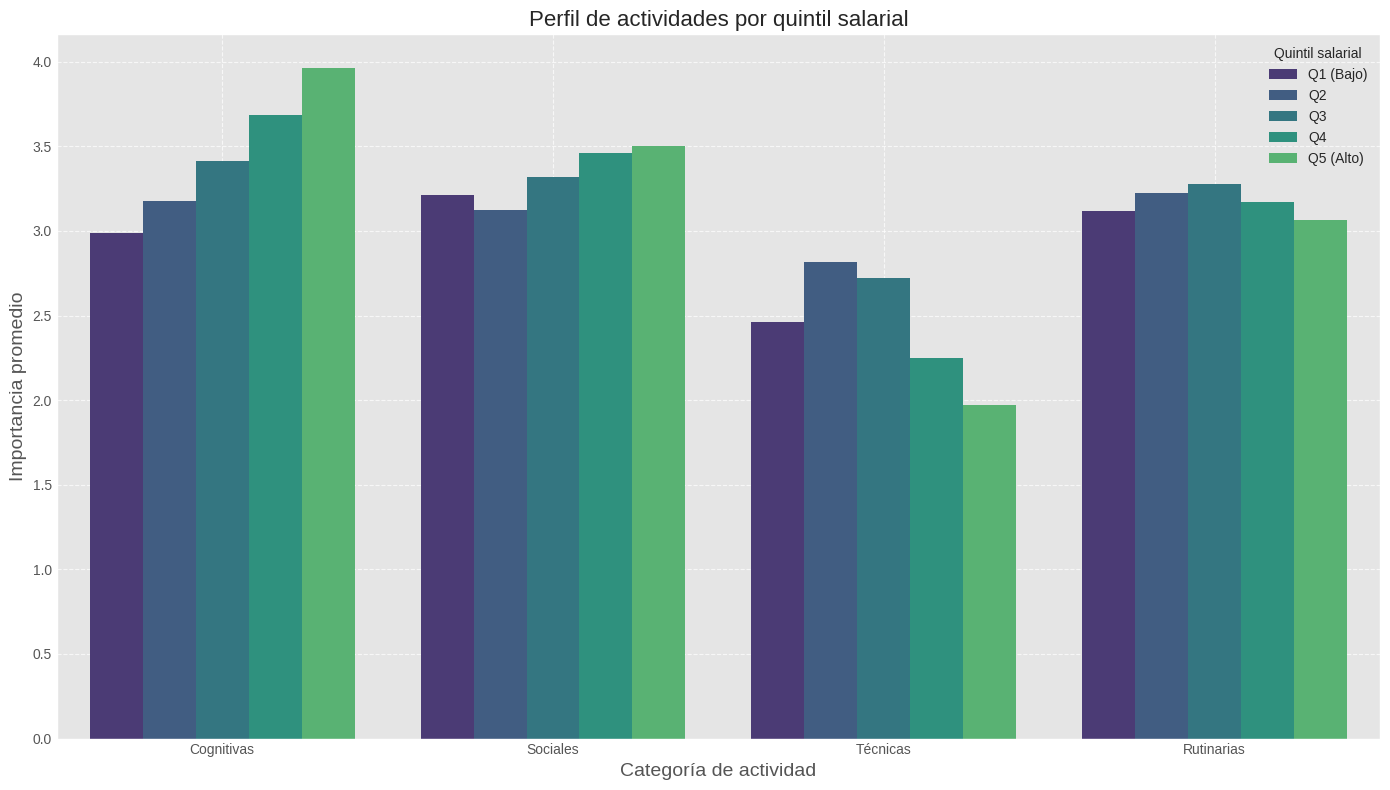
\includegraphics[width=0.8\textwidth]{views/entrega1/perfil_quintil_salarial.png}
    \caption{Perfil de actividades por quintil salarial}
    \label{fig:perfil_quintil}
\end{figure}

Este gráfico muestra una clara gradiente ascendente en la intensidad de actividades cognitivas a medida que aumenta el quintil salarial. Para el quintil superior (Q5), la intensidad media de actividades cognitivas alcanza 3.98 en una escala de 5, mientras que para el quintil más bajo (Q1) es de 2.98. Las actividades técnicas muestran la tendencia inversa, siendo menos importantes en los quintiles superiores.

\paragraph{Visualización 2: Relación entre Importancia de Actividades Cognitivas y Salario}
\begin{figure}[H]
    \centering
    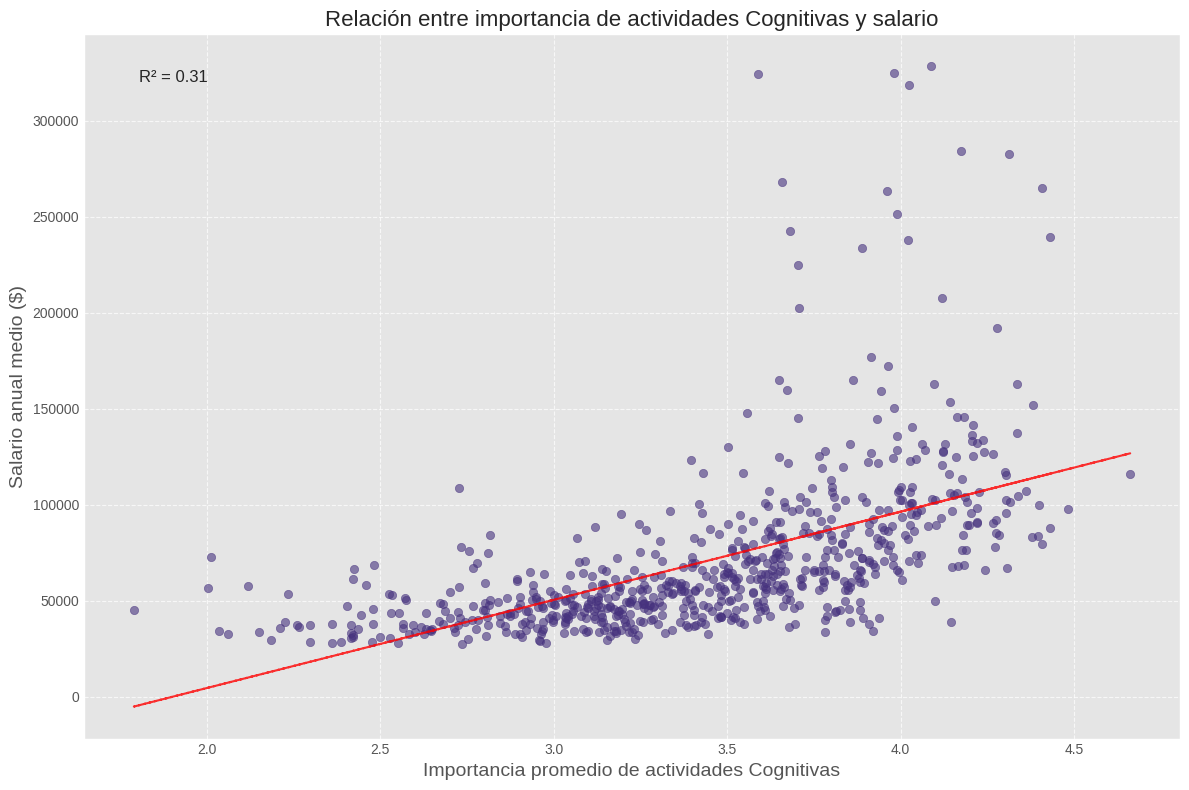
\includegraphics[width=0.8\textwidth]{views/entrega1/relacion_cognitivas_salario.png}
    \caption{Relación entre importancia de actividades cognitivas y salario}
    \label{fig:cognitivas_salario}
\end{figure}

El diagrama de dispersión demuestra la relación entre la intensidad de actividades cognitivas y el salario anual medio, con un coeficiente de determinación $R^2 = 0.31$, indicando que aproximadamente un tercio de la varianza salarial puede explicarse por la intensidad de actividades cognitivas.

\paragraph{Visualización 3: Correlación entre Categorías de Actividades y Salario}
\begin{figure}[H]
    \centering
    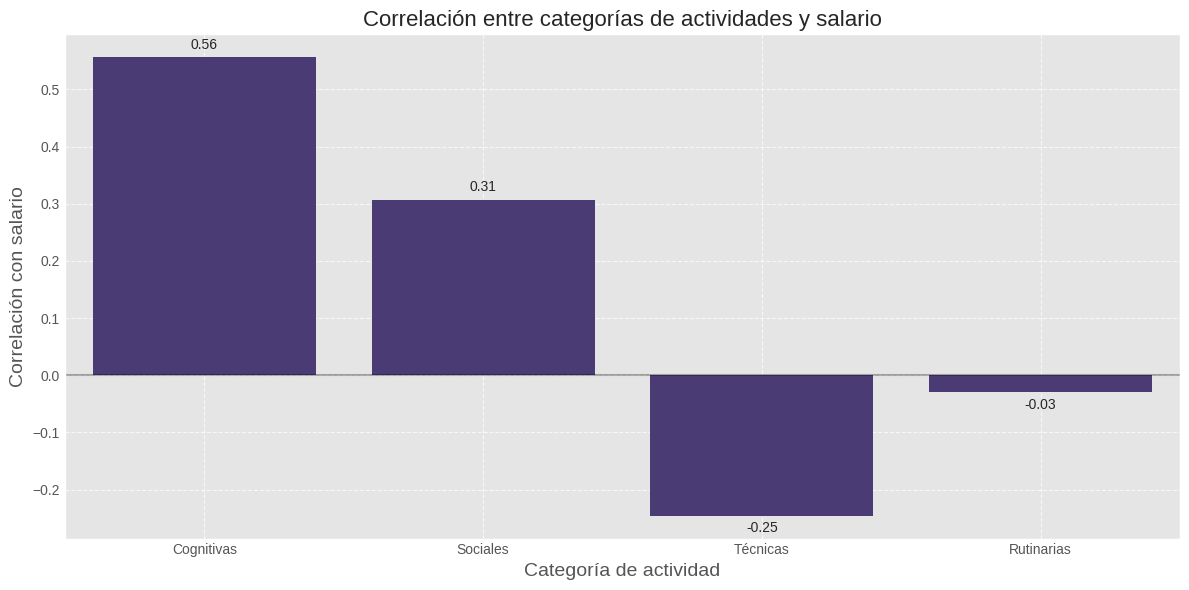
\includegraphics[width=0.8\textwidth]{views/entrega1/correlacion_categorias}
    \caption{Correlación entre categorías de actividades y salario}
    \label{fig:corr_categorias}
\end{figure}

El gráfico de barras ilustra la magnitud y dirección de las correlaciones entre las cuatro categorías de actividades y el salario anual medio, confirmando visualmente las diferencias significativas entre categorías.

\paragraph{Visualización 4: Actividades con Mayor Correlación con Salarios}
\begin{figure}[H]
    \centering
    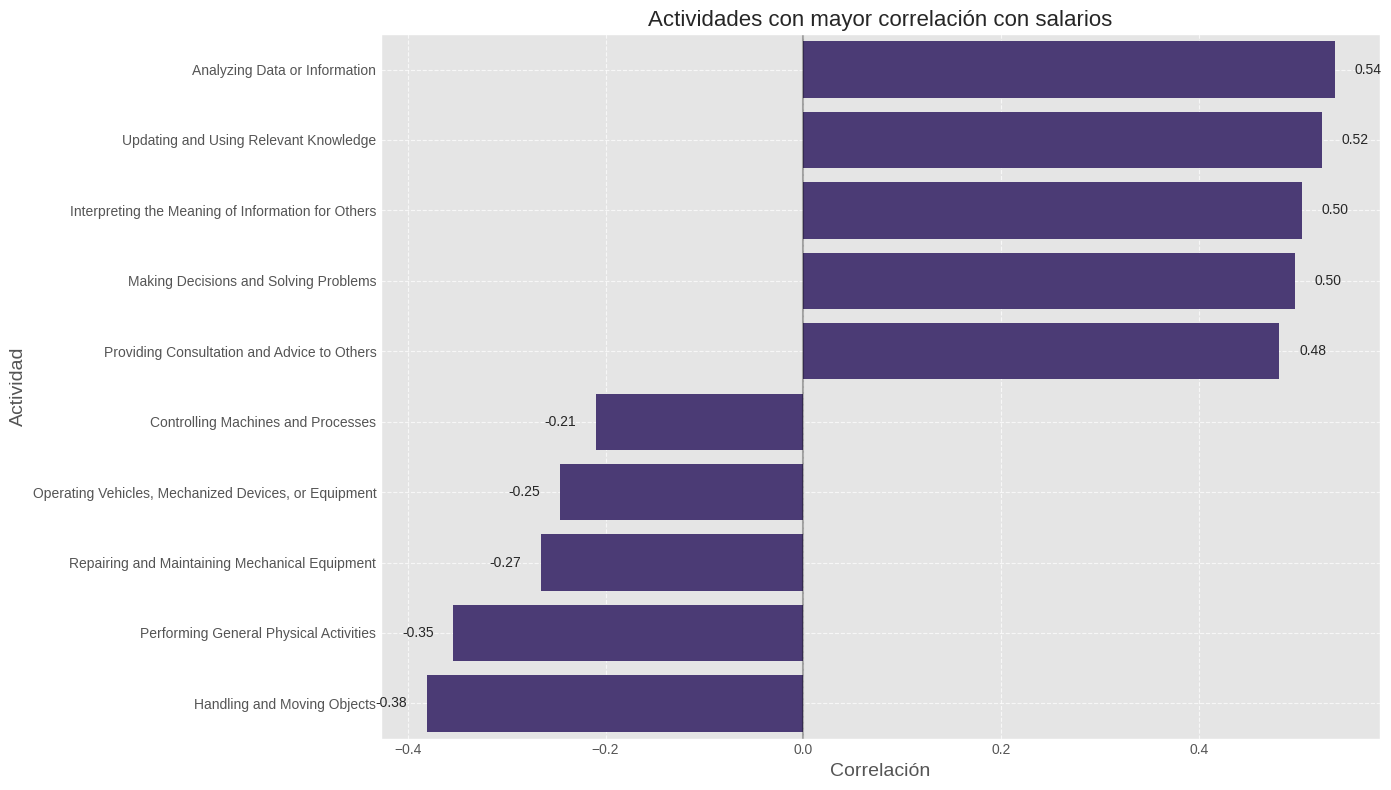
\includegraphics[width=0.8\textwidth]{views/entrega1/actividades_mayor_correlacion}
    \caption{Actividades con mayor correlación con salarios}
    \label{fig:actividades_correlacion}
\end{figure}

Este gráfico identifica las actividades específicas con las correlaciones más fuertes (positivas y negativas) con los salarios, demostrando el contraste entre actividades cognitivas/analíticas y actividades manuales/técnicas.

\paragraph{Visualización 5: Las 15 Actividades más Importantes en Promedio}
\begin{figure}[H]
    \centering
    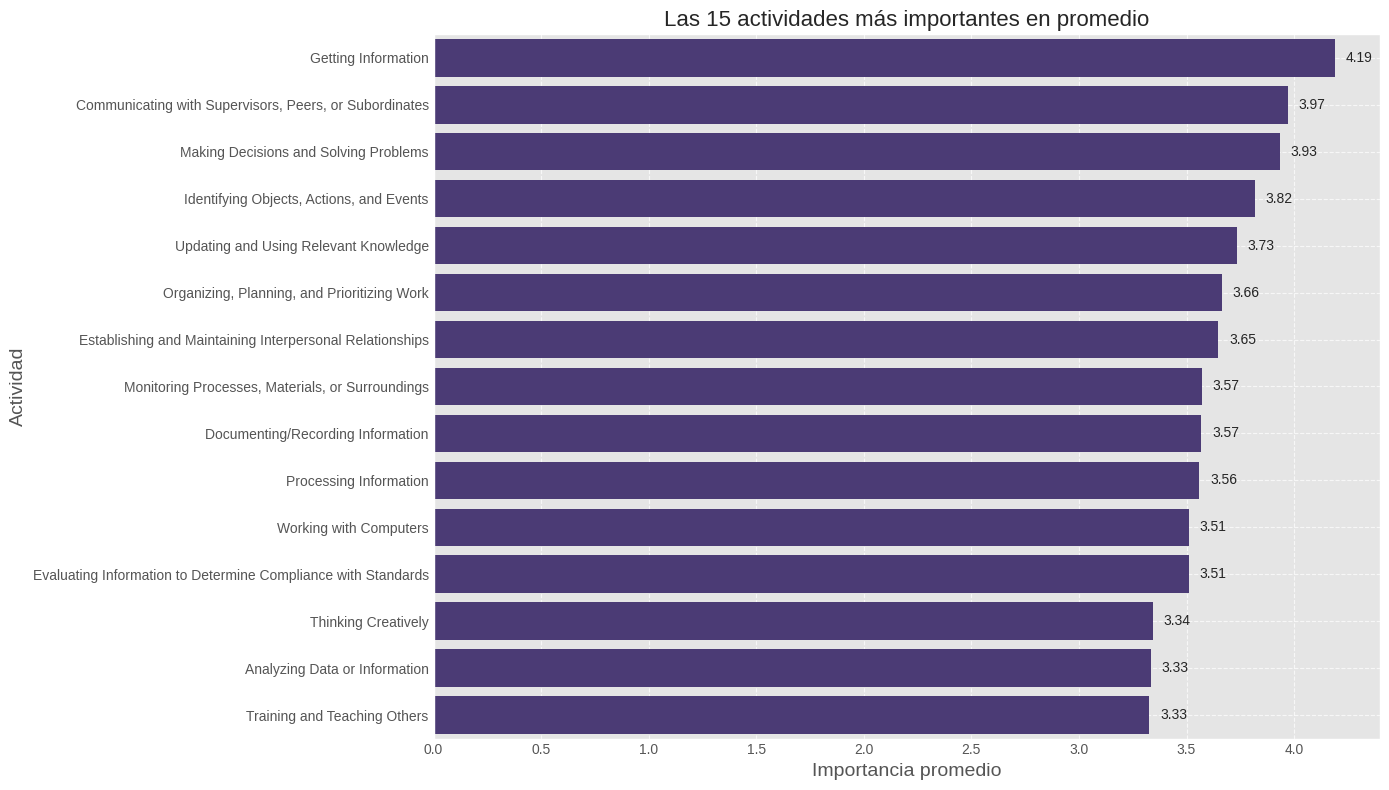
\includegraphics[width=0.8\textwidth]{views/entrega1/actividades_importantes}
    \caption{Las 15 actividades más importantes en promedio}
    \label{fig:actividades_importantes}
\end{figure}

Este gráfico muestra la prevalencia general de distintos tipos de actividades en el mercado laboral estadounidense, con ``Getting Information'' (4.19), ``Communicating with Supervisors, Peers, or Subordinates'' (3.97) y ``Making Decisions and Solving Problems'' (3.93) como las actividades más importantes en promedio.

Estos patrones empíricos sugieren un vínculo sistemático entre la naturaleza de las actividades laborales y los resultados económicos (medidos por los salarios), que podría fundamentar nuestro análisis teórico sobre la complementariedad trabajo-tecnología como mecanismo de crecimiento económico inclusivo.

\end{tcolorbox}

\subsubsection{[20 puntos] Exploración de Mecanismos Teóricos}

Proponga al menos un mecanismo teórico que vincule su dimensión elegida con el crecimiento económico (e.g. los nuevos inventos producen bienes únicos, por lo que las firmas que innovan tienen beneficios monopolísticos que duran hasta que alguien más haya inventado un bien nuevo (Aghion y Howitt, 1992). Esas utilidades incentivaran a otras empresas a gastar recursos en innovar). Si es capaz de pensar en más de un mecanismo teórico, discuta cuál de ellos es más relevante y por qué. Describa los agentes clave involucrados (por ejemplo, hogares, empresas, gobiernos) y explique cómo toman decisiones dentro de este mecanismo. Describa un ``experimento mental'' sobre cómo un cambio en esta dimensión afectaría el crecimiento económico.

\begin{tcolorbox}
\textbf{La Complementariedad Dinámica entre Capital Humano y Tecnología en el sector Servicios} 

Proponemos como mecanismo teórico central la ``complementariedad dinámica entre capital humano específico y tecnología en servicios cognitivos'' como motor de crecimiento económico inclusivo. A diferencia de los modelos tradicionales donde la tecnología tiende a sustituir trabajo por capital (especialmente en manufacturas), este mecanismo destaca cómo, en servicios intensivos en actividades cognitivas y sociales, la tecnología y el trabajo humano actúan como complementos estratégicos que se refuerzan mutuamente, generando un ciclo virtuoso de acumulación de habilidades, innovación, y crecimiento compartido de la productividad y los salarios.

Este mecanismo se fundamenta en la evidencia empírica presentada anteriormente, que muestra una fuerte correlación positiva entre la intensidad de actividades cognitivas/sociales y los niveles salariales ($r = 0.56$ y $r = 0.31$, respectivamente), mientras que las actividades técnicas fácilmente automatizables muestran correlaciones negativas ($r = -0.25$). Esta asimetría sugiere que las tecnologías contemporáneas son complementarias al trabajo humano en ciertas actividades, mientras que lo sustituyen en otras. \\

\textbf{Agentes y sus Decisiones}

\paragraph{1. Trabajadores}
Los trabajadores son agentes heterogéneos que maximizan su utilidad intertemporal tomando decisiones sobre:

\begin{itemize}
\item \textbf{Inversión en capital humano específico}: Eligen cuánto tiempo y recursos destinar a adquirir habilidades cognitivas y sociales complejas ($h$)
\item \textbf{Elección ocupacional}: Seleccionan entre ocupaciones intensivas en diferentes tipos de actividades
\end{itemize}

Formalmente, cada trabajador resuelve el siguiente problema:

\begin{align}
\max_{h} U = u(c_1) + \beta E[u(c_2)]
\end{align}

Sujeto a:
\begin{itemize}
\item $c_1 + e(h) = w_0$
\item $c_2 = \max\{w_s(h,T), w_m\}$
\end{itemize}

Donde:
\begin{itemize}
\item $c_1, c_2$ son consumo en períodos 1 y 2
\item $e(h)$ es el costo de educación, creciente y convexo en $h$
\item $w_0$ es un ingreso inicial
\item $w_s(h,T)$ es el salario en servicios cognitivos, función de habilidades $h$ y tecnología $T$
\item $w_m$ es el salario alternativo en manufacturas
\item $\beta$ es factor de descuento
\end{itemize}

La condición de primer orden clave es:

\begin{align}
e'(h) = \beta \frac{\partial w_s(h,T)}{\partial h}
\end{align}

Esta ecuación muestra que los trabajadores invertirán en habilidades específicas hasta que el costo marginal de educación iguale el valor presente descontado del retorno marginal a esas habilidades.

\paragraph{2. Empresas de Servicios}
Las empresas de servicios maximizan beneficios decidiendo:

\begin{itemize}
\item \textbf{Adopción tecnológica}: Invierten en tecnologías complementarias al trabajo cognitivo ($T$)
\item \textbf{Demanda de trabajo calificado}: Contratan trabajadores con habilidades específicas ($h$)
\item \textbf{Organización productiva}: Diseñan procesos que combinan óptimamente tecnología y habilidades
\end{itemize}

Formalmente, resuelven:

\begin{align}
\max_{L,T} \Pi_s = P_s \cdot A(T) \cdot F(h \cdot L, T) - w_s(h) \cdot L - r \cdot T
\end{align}

Donde:
\begin{itemize}
\item $P_s$ es el precio del servicio
\item $A(T)$ es productividad aumentadora, creciente en $T$
\item $F(h \cdot L, T)$ es una función de producción con complementariedad cruzada $\frac{\partial^2 F}{\partial (hL) \partial T} > 0$
\item $L$ es cantidad de trabajo
\item $r$ es costo de capital tecnológico
\end{itemize}

Las condiciones de primer orden son:

\begin{align}
\frac{\partial \Pi_s}{\partial L} &= P_s \cdot A(T) \cdot \frac{\partial F}{\partial (hL)} \cdot h - w_s(h) = 0\\
\frac{\partial \Pi_s}{\partial T} &= P_s \cdot \frac{\partial A(T)}{\partial T} \cdot F + P_s \cdot A(T) \cdot \frac{\partial F}{\partial T} - r = 0
\end{align}

Estas condiciones implican que las empresas contratarán trabajo hasta que su producto marginal iguale su costo, y adoptarán tecnología hasta que los beneficios marginales (tanto por aumento general de productividad como por complementariedad específica) igualen su costo marginal.

\paragraph{3. Empresas Manufactureras}
Las empresas manufactureras operan con una tecnología diferente:

\begin{align}
\max_{L_m,K} \Pi_m = P_m \cdot G(K, L_m) - w_m \cdot L_m - r_k \cdot K
\end{align}

Donde:
\begin{itemize}
\item $G(K, L_m)$ es una función de producción donde capital y trabajo son más sustitutivos
\item $K$ es capital físico que puede automatizar tareas
\item $L_m$ es trabajo manufacturero, menos especializado
\item $r_k$ es costo del capital físico
\end{itemize}

\paragraph{4. Instituciones Educativas}
Las instituciones educativas producen capital humano específico:

\begin{itemize}
\item Adaptan programas para desarrollar habilidades demandadas
\item Responden a señales de mercado sobre retornos a diferentes tipos de habilidades
\item Minimizan costos de producción de capital humano
\end{itemize}

Su función objetivo puede representarse como:

\begin{align}
\min_{x} C(h, x) \text{ s.t. } H(x) \geq \bar{h}
\end{align}

Donde:
\begin{itemize}
\item $C(h, x)$ es la función de costo
\item $x$ son insumos educativos
\item $H(x)$ es la función de producción de capital humano
\item $\bar{h}$ es un nivel mínimo requerido de calidad
\end{itemize}

\paragraph{5. Gobierno}
El gobierno establece políticas que afectan el equilibrio:

\begin{itemize}
\item Inversión en infraestructura digital y educativa
\item Regulación de mercados laborales y tecnológicos
\item Política fiscal y subsidios a formación e innovación
\end{itemize}

Su función objetivo puede incluir tanto eficiencia como equidad:

\begin{align}
\max_{g,\tau} W = \int_i \alpha_i U_i(g, \tau) di
\end{align}

Donde:
\begin{itemize}
\item $W$ es bienestar social
\item $g$ son gastos públicos
\item $\tau$ son impuestos
\item $\alpha_i$ son ponderaciones de bienestar
\end{itemize}

\textbf{Equilibrio y Dinámica}

El equilibrio en este modelo implica interacciones complejas entre decisiones de los agentes:

\begin{enumerate}
\item Los trabajadores invierten en capital humano anticipando salarios futuros
\item Las empresas adoptan tecnología y demandan habilidades específicas
\item Las instituciones educativas producen capital humano respondiendo a señales de mercado
\item El gobierno establece políticas que afectan los incentivos
\end{enumerate}

La dinámica clave que genera crecimiento sostenido es la retroalimentación positiva entre acumulación de capital humano específico y adopción de tecnología complementaria:

\begin{align}
\frac{\partial w_s(h,T)}{\partial h \partial T} > 0
\end{align}

Esta derivada cruzada positiva implica que el retorno marginal a las habilidades aumenta con el nivel tecnológico, y viceversa. Algebraicamente, esto genera un sistema dinámico donde tanto $h$ como $T$ crecen endógenamente a lo largo del tiempo:

\begin{align}
h_{t+1} &= \Phi(h_t, T_t)\\
T_{t+1} &= \Psi(h_t, T_t)
\end{align}

Con $\frac{\partial \Phi}{\partial T} > 0$ y $\frac{\partial \Psi}{\partial h} > 0$, lo que implica retornos crecientes a escala a nivel agregado.

En contraste, en el sector manufacturero, la relación entre automatización y trabajo es predominantemente sustitutiva:

\begin{align}
\frac{\partial w_m(K)}{\partial K} < 0
\end{align}

Esto genera divergencia sectorial en productividad y salarios, impulsando cambio estructural.

\subsubsection*{Mecanismos Específicos de Transmisión}

\begin{enumerate}
\item \textbf{Efecto de señalización}: Los salarios más altos en actividades cognitivas señalizan a los trabajadores que deben invertir en estas habilidades:
\begin{align}
\frac{\partial h}{\partial (w_s/w_m)} > 0
\end{align}

\item \textbf{Efecto de escala}: Mayor capital humano aumenta el tamaño potencial del mercado para tecnologías complementarias:
\begin{align}
\frac{\partial T}{\partial h} > 0 \text{ debido a } \frac{\partial \Pi_T}{\partial h} > 0
\end{align}

\item \textbf{Efecto de innovación inducida}: La complementariedad dirige el esfuerzo innovador hacia tecnologías que aumentan la productividad del trabajo cognitivo:
\begin{align}
\frac{\partial \dot{A}}{\partial (w_s \cdot h \cdot L)} > 0
\end{align}

\item \textbf{Efecto de aprendizaje}: El uso de tecnologías avanzadas aumenta la capacidad de los trabajadores para adquirir habilidades adicionales:
\begin{align}
\frac{\partial \dot{h}}{\partial T} > 0
\end{align}

\item \textbf{Efecto de externalidades de conocimiento}: La concentración de trabajadores calificados genera spillovers productivos:
\begin{align}
A_i = \bar{A} \cdot \left( \frac{h_i}{\bar{h}} \right)^\gamma \text{ con } \gamma > 0
\end{align}

\end{enumerate}

\textbf{Experimento Mental: Dos Trayectorias de Desarrollo}

Consideremos dos economías inicialmente idénticas que experimentan un shock tecnológico similar (avance en IA y automatización), pero siguen diferentes estrategias de adaptación:

\paragraph{Economía A: Enfoque en Preservación Industrial}
La Economía A implementa políticas para proteger y preservar su base manufacturera tradicional:
\begin{itemize}
\item Subsidios al capital físico: reduce $r_k$
\item Protección comercial: aumenta artificialmente $P_m$
\item Descuida inversión en educación superior: mantiene alto $e(h)$ para habilidades cognitivas avanzadas
\end{itemize}

Resultados a mediano plazo:
\begin{enumerate}
\item Nivel de automatización manufacturera artificialmente bajo
\item Desincentivos a inversión en capital humano específico
\item Menor adopción de tecnologías complementarias
\item Estancamiento salarial generalizado
\item Productividad agregada limitada
\item Crecimiento económico lento y desigual
\end{enumerate}

La ecuación de crecimiento resultante sería:
\begin{align}
g_A = \alpha \cdot \left( \frac{\dot{K}}{K} \right) + (1-\alpha) \cdot \left( \frac{\dot{L}}{L} \right) + \dot{A}_0
\end{align}

Con una tasa de progreso técnico $\dot{A}_0$ exógena y baja.

\paragraph{Economía B: Enfoque en Servicios Cognitivos}
La Economía B reorienta su estrategia hacia el desarrollo de servicios intensivos en actividades cognitivas:
\begin{itemize}
\item Inversión en educación superior y formación continua: reduce $e(h)$
\item Infraestructura digital: reduce costos fijos de adopción tecnológica
\item Política industrial enfocada en servicios avanzados: promueve $P_s$
\item Regulación favorable a complementariedad trabajo-tecnología
\end{itemize}

Resultados a mediano plazo:
\begin{enumerate}
\item Rápida acumulación de capital humano específico
\item Alta adopción de tecnologías complementarias
\item Círculo virtuoso entre habilidades e innovación
\item Crecimiento salarial inclusivo
\item Aumento sostenido de productividad
\item Crecimiento económico dinámico y compartido
\end{enumerate}

La ecuación de crecimiento resultante sería:
\begin{align}
g_B = \alpha \cdot \left( \frac{\dot{K}}{K} \right) + (1-\alpha) \cdot \left( \frac{\dot{L}}{L} \right) + \dot{A}(h,T)
\end{align}

Con una tasa de progreso técnico endógena $\dot{A}(h,T)$ que aumenta con la acumulación simultánea de capital humano específico y tecnología complementaria.

\paragraph{Comparación Dinámica}
Inicialmente, la Economía A podría mantener mayor nivel de empleo manufacturero, pero con el tiempo la Economía B desarrollaría:
\begin{itemize}
\item Mayor valor agregado por trabajador
\item Salarios más altos y más uniformemente distribuidos
\item Mayor resistencia a shocks tecnológicos
\item Crecimiento más sostenible a largo plazo
\end{itemize}

Este resultado se debe fundamentalmente a que la Economía B aprovecha la complementariedad entre capital humano específico y tecnología en servicios cognitivos, generando un ciclo virtuoso de innovación y desarrollo de habilidades que sostiene el crecimiento inclusivo.

Algebraicamente, la diferencia clave es:
\begin{align}
\lim_{t \to \infty} \frac{Y_B(t)}{Y_A(t)} = \lim_{t \to \infty} e^{\int_0^t [g_B(s) - g_A(s)] ds} = \lim_{t \to \infty} e^{\int_0^t [\dot{A}(h,T) - \dot{A}_0] ds} = \infty
\end{align}

Si $\dot{A}(h,T) > \dot{A}_0$ para todo $t$, lo que implica divergencia en el largo plazo.

Este mecanismo teórico se alinea con los patrones empíricos identificados previamente, en los que la intensidad de las actividades cognitivas exhibe una fuerte correlación positiva con los salarios, mientras que las actividades técnicas fácilmente automatizables muestran una correlación negativa. El experimento mental demuestra cómo distintas respuestas políticas frente al mismo shock tecnológico pueden resultar en trayectorias de desarrollo radicalmente diferentes, con implicaciones clave para el crecimiento económico inclusivo.

\end{tcolorbox}

\subsubsection{[20 puntos] De los conceptos a la teoría}

Describa en palabras cómo modelaría las dinámicas que describió en el apartado anterior. Distinga explícitamente entre:
\begin{enumerate}
\item Supuestos de comportamiento: ¿cómo es el proceso de toma de decisiones de los agentes?
\item Condiciones de equilibrio: ¿Cómo interactúan los agentes? Cómo se compaginan las decisiones individuales para determinar resultados agregados.
\end{enumerate}

\begin{tcolorbox}

Para formalizar el mecanismo de complementariedad dinámica entre capital humano específico y cambios tecnológicos, proponemos desarrollar un modelo de equilibrio general dinámico con dos sectores productivos (servicios cognitivos y manufactura) y agentes heterogéneos. A continuación, describimos en detalle los componentes fundamentales de este modelo.

\textbf{1. Supuestos de comportamiento}

\paragraph{1.1 Trabajadores}
Los trabajadores son agentes heterogéneos que viven durante dos períodos y toman decisiones secuenciales:

\begin{itemize}
\item \textbf{Período 1 (juventud)}: Deciden cuánto invertir en capital humano específico
\item \textbf{Período 2 (adultez)}: Eligen el sector de empleo y ofrecen trabajo
\end{itemize}

Formalmente, cada trabajador resuelve el siguiente problema de maximización:

\begin{align}
\max_{h} U(c_1, c_2) = u(c_1) + \beta \mathbb{E}[u(c_2)]
\end{align}

Donde:
\begin{itemize}
\item $c_1 = y_1 - e(h)$ es el consumo en el período 1
\item $y_1$ es un ingreso inicial exógeno
\item $e(h)$ es el costo de educación, una función creciente y estrictamente convexa de $h$
\item $c_2 = \max\{w_s(h,T), w_m\}$ es el consumo en el período 2
\item $w_s(h,T)$ es el salario en el sector de servicios, que depende positivamente de $h$ y $T$
\item $w_m$ es el salario en el sector manufacturero
\item $\beta$ es el factor de descuento intertemporal
\item $u(\cdot)$ es una función de utilidad cóncava estándar con $u' > 0$, $u'' < 0$, y que satisface las condiciones de Inada
\end{itemize}

Supuestos adicionales sobre el comportamiento:
\begin{itemize}
\item Los trabajadores tienen expectativas racionales sobre los salarios futuros
\item Existe heterogeneidad en las habilidades innatas ($\theta_i$) que afectan el costo de adquisición de capital humano: $e(h,\theta_i)$ con $\frac{\partial e}{\partial \theta_i} < 0$
\item La decisión sectorial en el período 2 sigue una regla simple de maximización de ingresos
\end{itemize}

\paragraph{1.2 Empresas de Servicios Cognitivos}
Las empresas en este sector utilizan trabajo calificado y tecnología como insumos complementarios. Cada empresa maximiza beneficios:

\begin{align}
\max_{L_s,T} \Pi_s = P_s \cdot Y_s - w_s(h) \cdot L_s - r_T \cdot T
\end{align}

Donde:
\begin{itemize}
\item $Y_s = A_s(T) \cdot F(h \cdot L_s, T)$ es la función de producción
\item $A_s(T)$ es un factor de productividad que aumenta con el nivel tecnológico: $A_s'(T) > 0$
\item $F(\cdot,\cdot)$ es una función de producción con rendimientos constantes a escala
\item $L_s$ es la cantidad de trabajadores empleados
\item $h$ es el nivel promedio de capital humano específico de los trabajadores contratados
\item $P_s$ es el precio del bien de servicios
\item $r_T$ es el costo de la tecnología
\item $F$ exhibe complementariedad estratégica: $\frac{\partial^2 F}{\partial (hL_s) \partial T} > 0$
\end{itemize}

Supuestos adicionales sobre el comportamiento:
\begin{itemize}
\item Las empresas actúan como tomadoras de precios en todos los mercados
\item La tecnología $T$ es divisible y puede ajustarse sin costos de ajuste
\item Las empresas tienen expectativas racionales sobre la oferta y calidad del trabajo
\end{itemize}

\paragraph{1.3 Empresas Manufactureras}
Las empresas manufactureras utilizan trabajo menos calificado y capital físico, con mayor sustituibilidad entre factores:

\begin{align}
\max_{L_m,K} \Pi_m = P_m \cdot Y_m - w_m \cdot L_m - r_K \cdot K
\end{align}

Donde:
\begin{itemize}
\item $Y_m = A_m \cdot G(K, L_m)$ es la función de producción
\item $A_m$ es la productividad manufacturera
\item $G(\cdot,\cdot)$ es una función de producción con rendimientos constantes a escala
\item $L_m$ es la cantidad de trabajadores empleados
\item $K$ es el capital físico, que puede automatizar tareas rutinarias
\item $P_m$ es el precio del bien manufacturado
\item $r_K$ es el rendimiento del capital físico
\item $G$ exhibe mayor elasticidad de sustitución que $F$: $\sigma_G > \sigma_F$
\end{itemize}

Supuestos adicionales sobre el comportamiento:
\begin{itemize}
\item La automatización desplaza trabajo: $\frac{\partial L_m}{\partial K} < 0$ para un nivel dado de producción
\item Las empresas manufactureras también son tomadoras de precios
\item El capital físico $K$ es perfectamente divisible
\end{itemize}

\paragraph{1.4 Sector de Investigación y Desarrollo (I+D)}
Este sector produce innovaciones tecnológicas siguiendo:

\begin{align}
\max_{R_T} \Pi_{I+D} = V(T) - C(R_T)
\end{align}

Donde:
\begin{itemize}
\item $V(T)$ es el valor presente de los beneficios de innovar
\item $C(R_T)$ es el costo de I+D
\item $\dot{T} = \phi(R_T, h)$ es la ecuación de movimiento de la tecnología
\item $\phi$ es creciente en ambos argumentos: $\frac{\partial \phi}{\partial R_T} > 0$, $\frac{\partial \phi}{\partial h} > 0$
\end{itemize}

Supuesto clave: la productividad de la I+D aumenta con el nivel de capital humano específico disponible en la economía, capturando spillovers de conocimiento.

\paragraph{1.5 Instituciones Educativas}
Las instituciones educativas producen capital humano específico minimizando costos:

\begin{align}
\min_{x} C(h, x)
\end{align}

Sujeto a:
\begin{itemize}
\item $H(x) \geq \bar{h}$
\item $C(h,x)$ es la función de costo educativo
\item $x$ es un vector de insumos educativos
\item $H(x)$ es la función de producción de capital humano
\item $\bar{h}$ es un nivel mínimo exigido de calidad
\end{itemize}

Supuestos adicionales:
\begin{itemize}
\item Las instituciones responden a incentivos de mercado
\item Existen economías de escala en la producción de capital humano
\item Los programas educativos se adaptan a la demanda laboral con cierto rezago
\end{itemize}

\textbf{2. Condiciones de equilibrio}

\paragraph{2.1 Equilibrio en el Mercado Laboral}
El equilibrio en el mercado laboral requiere que:

\begin{enumerate}
\item La oferta de trabajo iguale a la demanda en cada sector:
\begin{align}
L_s^S(w_s, w_m, h) &= L_s^D(w_s, r_T, T, P_s)\\
L_m^S(w_s, w_m, h) &= L_m^D(w_m, r_K, K, P_m)
\end{align}

\item Condición de indiferencia para el trabajador marginal:
\begin{align}
w_s(h^*, T) = w_m
\end{align}
Donde $h^*$ es el nivel de capital humano específico del trabajador indiferente entre sectores.

\item Curva de salarios creciente en capital humano en servicios:
\begin{align}
\frac{\partial w_s(h,T)}{\partial h} > 0 \text{ para todo } h
\end{align}

\item Sorting positivo: los trabajadores con mayor capital humano específico ($h > h^*$) elegirán el sector de servicios cognitivos, mientras que aquellos con menor capital humano ($h < h^*$) elegirán el sector manufacturero.
\end{enumerate}

\paragraph{2.2 Equilibrio en el Mercado de Bienes}
El equilibrio en el mercado de bienes requiere que la oferta iguale a la demanda en ambos sectores:

\begin{align}
Y_s &= C_s + X_s\\
Y_m &= C_m + I_K + X_m
\end{align}

Donde:
\begin{itemize}
\item $C_s$ y $C_m$ son el consumo de servicios y manufacturas
\item $X_s$ y $X_m$ son exportaciones netas
\item $I_K$ es inversión en capital físico
\end{itemize}

La demanda relativa de bienes sigue una relación con precios relativos y nivel de ingreso:

\begin{align}
\frac{C_s}{C_m} = \Omega\left(\frac{P_m}{P_s}, Y\right)
\end{align}

Con $\frac{\partial \Omega}{\partial (P_m/P_s)} < 0$ y $\frac{\partial \Omega}{\partial Y} > 0$ si los servicios cognitivos son bienes superiores.

\paragraph{2.3 Equilibrio en el Mercado de Capital}
El equilibrio en el mercado de capital requiere:

\begin{enumerate}
\item Igualdad entre oferta y demanda de capital físico:
\begin{align}
K^S(r_K) = K^D(r_K, w_m, P_m)
\end{align}

\item Igualdad entre oferta y demanda de capital tecnológico:
\begin{align}
T^S(r_T, h) = T^D(r_T, w_s, h, P_s)
\end{align}

\item Condición de arbitraje entre inversiones:
\begin{align}
r_K = r_T = r + \delta + \rho
\end{align}
Donde $r$ es la tasa de interés real, $\delta$ es la tasa de depreciación, y $\rho$ es la prima de riesgo.
\end{enumerate}

\paragraph{2.4 Equilibrio Dinámico}
El equilibrio dinámico del sistema está caracterizado por las siguientes ecuaciones de movimiento:

\begin{enumerate}
\item Acumulación de capital humano específico:
\begin{align}
\dot{h} = \psi(e(h), T)
\end{align}
Con $\frac{\partial \psi}{\partial e} > 0$ y $\frac{\partial \psi}{\partial T} > 0$, capturando el efecto de aprendizaje por uso de tecnologías avanzadas.

\item Evolución tecnológica:
\begin{align}
\dot{T} = \phi(R_T, h)
\end{align}
Donde la productividad de I+D aumenta con el capital humano promedio.

\item Acumulación de capital físico:
\begin{align}
\dot{K} = I_K - \delta_K K
\end{align}
Donde $\delta_K$ es la tasa de depreciación del capital físico.

\item Productividad sectorial:
\begin{align}
\dot{A_s} &= \lambda_s(T, h) \cdot A_s\\
\dot{A_m} &= \lambda_m(K) \cdot A_m
\end{align}
Con $\lambda_s$ más sensible a la complementariedad entre capital humano y tecnología.
\end{enumerate}

\paragraph{2.5 Estado Estacionario}
En el estado estacionario se cumple:
\begin{itemize}
\item $\dot{h} = \dot{T} = \dot{K} = 0$
\item Crecimiento balanceado: $\frac{\dot{Y}}{Y} = \frac{\dot{A_s}}{A_s} = \frac{\dot{A_m}}{A_m} = g^*$
\item Precios relativos estables: $\frac{\dot{P_s}}{P_s} = \frac{\dot{P_m}}{P_m}$
\item Distribución estable de trabajadores entre sectores
\end{itemize}

La tasa de crecimiento de estado estacionario $g^*$ dependerá crucialmente de la fuerza de la complementariedad entre capital humano específico y tecnología.

\paragraph{2.6 Equilibrio con Múltiples Estados Estacionarios}
Una característica importante del modelo es la posibilidad de múltiples equilibrios debido a la complementariedad estratégica entre acumulación de capital humano y desarrollo tecnológico.

Formalmente, pueden existir al menos tres estados estacionarios:

\begin{enumerate}
\item \textbf{Equilibrio de bajo nivel}:
\begin{itemize}
\item Bajo nivel de capital humano específico
\item Baja adopción tecnológica
\item Predominio del sector manufacturero
\item Crecimiento lento
\end{itemize}

\item \textbf{Equilibrio inestable intermedio}:
\begin{itemize}
\item Punto de inflexión que separa las cuencas de atracción de los equilibrios estables
\end{itemize}

\item \textbf{Equilibrio de alto nivel}:
\begin{itemize}
\item Alto nivel de capital humano específico
\item Alta adopción tecnológica
\item Predominio de servicios cognitivos
\item Crecimiento rápido e inclusivo
\end{itemize}
\end{enumerate}

La existencia de estos múltiples equilibrios justifica la intervención de política para ``empujar'' a la economía hacia el equilibrio superior.

\paragraph{2.7 Resultados Agregados}
Las decisiones individuales de los agentes se agregan para determinar:

\begin{enumerate}
\item \textbf{Productividad Total de Factores (TFP)}:
\begin{align}
TFP = [s_s \cdot A_s^{\rho} + s_m \cdot A_m^{\rho}]^{1/\rho}
\end{align}
Donde $s_s$ y $s_m$ son las participaciones sectoriales en el valor agregado.

\item \textbf{Distribución del ingreso}:
\begin{align}
Gini = \Gamma(w_s(h,T), w_m, L_s, L_m)
\end{align}
La desigualdad dependerá de los diferenciales salariales entre sectores y de la distribución de trabajadores.

\item \textbf{Crecimiento económico}:
\begin{align}
g = \alpha \cdot \left(\frac{\dot{K}}{K}\right) + (1-\alpha) \cdot \left(\frac{\dot{L}}{L}\right) + \left(\frac{\dot{TFP}}{TFP}\right)
\end{align}
Donde el crecimiento de la TFP está endógenamente determinado por la complementariedad dinámica entre capital humano específico y tecnología.

\item \textbf{Cambio estructural}:
\begin{align}
\frac{d(L_s/L)}{dt} = \Upsilon(h, T, P_s/P_m, Y)
\end{align}
La velocidad de cambio estructural depende del desarrollo de capital humano, tecnología, precios relativos y nivel de ingreso.
\end{enumerate}

Este marco teórico formaliza el mecanismo de complementariedad dinámica entre el capital humano específico y la tecnología en los servicios cognitivos, ofreciendo una base para examinar cómo diversas políticas y condiciones iniciales pueden llevar a trayectorias de desarrollo divergentes. La principal innovación en comparación con los modelos estándar de crecimiento radica en la endogeneización de la complementariedad tecnología-trabajo como impulsora de un desarrollo inclusivo, a diferencia de los modelos en los que la tecnología principalmente sustituye al trabajo.
\end{tcolorbox}

\nocite{*}

\printbibliography

\section*{Disclaimer}

Este documento fue producido con la asistencia de herramientas de inteligencia artificial (ChatGPT y Claude AI) para escribir el código LaTeX y para mejorar aspectos de redacción y claridad en las respuestas. Posterior a la utilización de estas herramientas, he revisado y editado cuidadosamente todo el contenido y asumo responsabilidad completa por el mismo.







\end{document}